% !TeX root = ../thuthesis-example.tex

\chapter{对称子段判定算法}

本章将对对称子段判定算法进行研究。根据第2章的定义,
对称子段指的是所有点关于
某个对称中心前后互为镜像的时间序列子段。
对称子段判定就是要通过计算给定子段的对称度,
判断子段是否具有对称性。
从数学意义上来说,对称子段判定算法是对称子段挖掘
算法的子问题,该算法不需要以子段长度$w$作为约束,直接度量
给定子段的对称性,并以对称度在阈值范围内的子段
作为对称子段。
因此,本章节的结构组织如下,在3.1节中分析了
基于对称中心与原始和反转时间序列相似性度量对称性的不足,
进而提出了基于最优匹配的单一对称性度量算法;在3.2节中根据时间序列子段的数据特征
提出了单一对称度阈值确定算法;在3.3节中利用对称度阈值对子段进行
分类,从而得到对称子段;并在3.4节中将对称子段判定算法扩展
到了流式数据领域。

\section{单一对称性度量算法}

对于单条时间序列子段而言,使用原始和反转时间序列的相似性来度量对称性,
是一种可行的对称性度量方法。此方法的好处是可以避免确定对称中心
的问题,但是,这种方法实际上是将子段对称中心两侧的部分进行了
两次匹配,不仅降低了对称性度量算法的时间效率,还增大了对称性的度量结果。
图~\ref{fig:beijing_temp}展示了在北京市历年月平均气温变化
时间序列中截取2010年的子段数据,显然,
气温时间序列子段具有对称性。但是,经计算,其原始和反转时间序列
的欧氏距离为16.67,而使用本文所提出的对称性度量方法,
气温时间序列子段的对称度仅为7.6,更加符合真实的子段对称性度量结果。
因此,本文定义了一种新的基于
最优匹配和区间动态规划思想的对称性度量方式,
既保证了准确率高、鲁棒性强的特点,
又提高了对称度的计算效率。
\begin{figure}
  \centering
  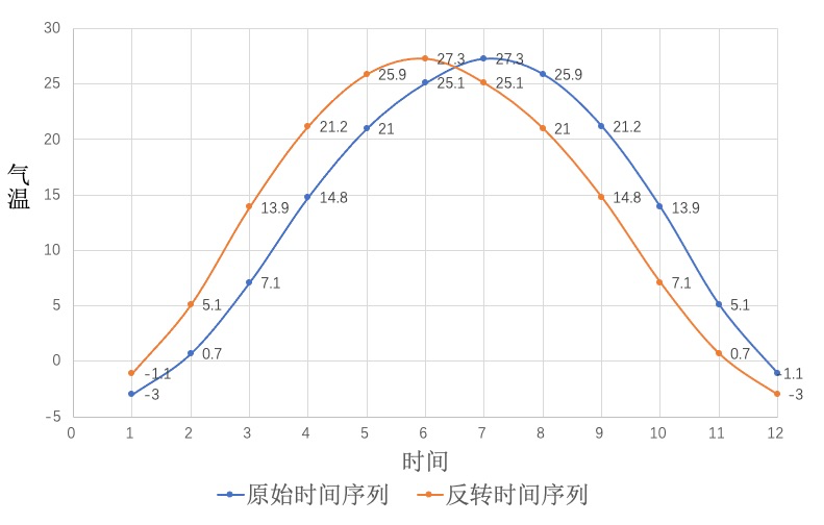
\includegraphics[width=0.76\linewidth]{beijing_temp.png}
  \caption{北京市2010年月平均气温变化}
  \label{fig:beijing_temp}
\end{figure}

为方便描述,本章将子段表示为单一时间序列形式。
首先从全局角度考虑对称子段的
匹配过程,由于不存在明确的对称中心,只能通过点和点之间的直接匹配度量
子段的对称性。由于子段的采集频率和位置不同,对于每个单点而言,
并不确定最佳匹配点的位置。尽管如此,如果一个时间序列子段是前后对称的,
那么首尾点一定是匹配的。图~\ref{fig:frontend_match}展示了
对称子段匹配过程的候选点,对于给定时间序列子段
$X=\left(\left(t_1,x_1 \right),\left(t_2,x_2\right),\dots,
  \left(t_n,x_n \right)\right)$而言,
第一个点$x_1$和最后一个点$x_n$是必然匹配的,但由于子段在
同一位置的持续时间不同,其他点如$x_2$和$x_{n-1}$等的匹配点却不是
唯一的,$x_2$可以一一对应地与$x_{n-1}$进行匹配,也可以通过扭曲时间
和$x_n$进行匹配,甚至可以与$x_{n-2},x_{n-3},\dots$等进行匹配,
而制约$x_2$与$x_k$匹配的条件不仅仅是这两点之间的距离,而是
时间序列子段$\left(\left(t_2,x_2 \right),\dots,\left(t_k,x_k \right)\right)$
的对称度。

\begin{figure}
  \centering
  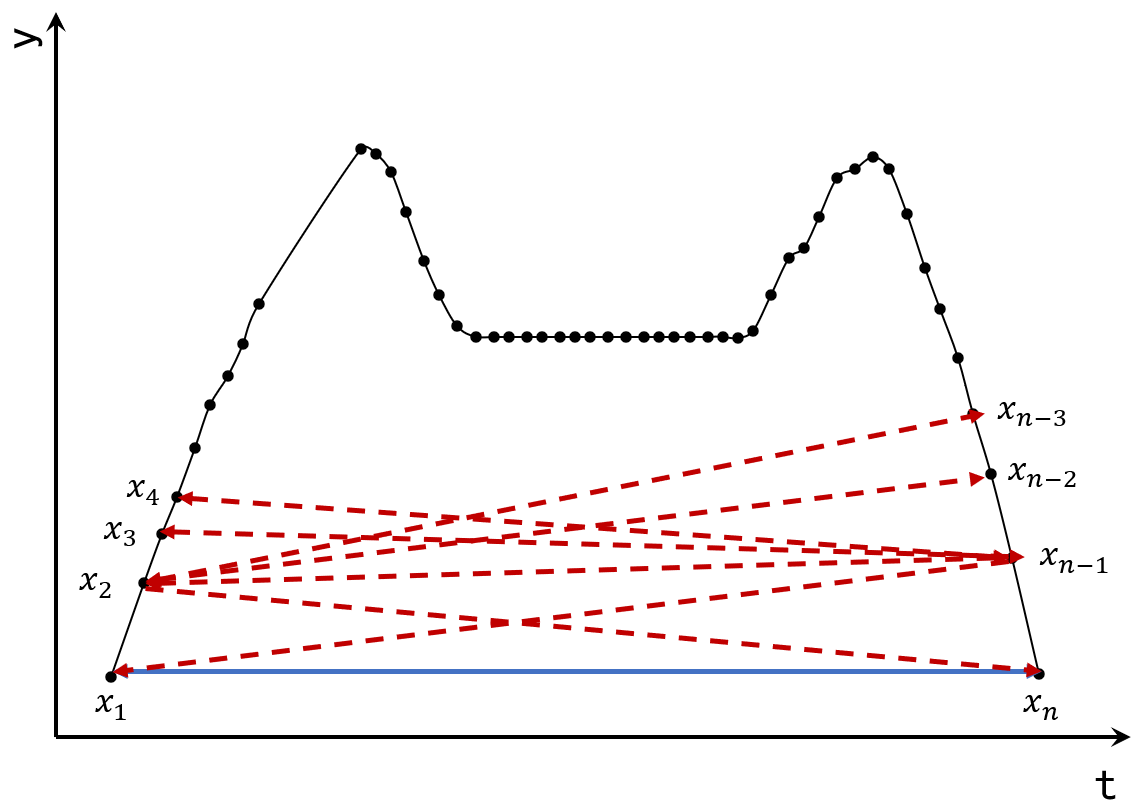
\includegraphics[width=0.70\linewidth]{frontend_match.png}
  \caption{对称子段首尾匹配候选点}
  \label{fig:frontend_match}
\end{figure}

接下来,本节将对时间序列子段的对称度算法进行标准的形式化推导。
对于单条时间序列子段$X=\left(\left(t_1,x_1 \right),\left(t_2,x_2\right),\dots,
  \left(t_n,x_n \right)\right)$,
计算每两个点之间的距离组成$n \times n$的
距离矩阵$D_{n \times n}$,矩阵中的每个元素由公式~\ref{eq:distance_matrix}计算而来
\begin{equation}
  D\left(i, j\right)=\left\|x_{i}-x_{j}\right\|_{w}
  \label{eq:distance_matrix}
\end{equation}

$D\left(i, j\right)$为点$p_i$与$p_j$间的距离,$i,j=1,2,\dots,n$。
显然,点$p_i$和$p_j$的匹配与$p_j$和$p_i$的匹配距离是相同的,
只是匹配顺序不同。为避免重复计算,本文只保留前点和后点的匹配,
则距离矩阵$D_{n \times n}$只需要计算反对角线以上的斜三角矩阵即可。
为了计算$X$的对称度,需要找到一条最优的匹配路径
$R_{best}=\left(r_1,r_2,\dots,r_k \right),\left⌊n/2\right⌋ \leq
  k < n$,使得$X$的匹配距离之和最小。 
其中,$r_k$为匹配路径中的第$k$个点,
若$r_k=\left(i,j\right)_k$,则其表示$p_i$与$p_j$之间的对称匹配。
由距离和路径的计算方式可知,距离矩阵中通常存在着多条
匹配路径,有效的匹配路径$R$要满足以下3个条件:
\begin{enumerate}
  \item 边界性:$r_{1} \in\{(i, i),(i, i+1) \mid 1 \leq i \leq n\}, \quad r_{k}=(1, n)$
  \item 单调性:给定$r_{k}=(i, j)$和$r_{k+1}=\left(i^{\prime}, j^{\prime}\right), \quad i^{\prime} \leq i, j^{\prime} \geq j$
  \item 连续性:给定$r_{k}=(i, j)$和$r_{k+1}=\left(i^{\prime}, j^{\prime}\right), \quad i^{\prime} \geq i-1, j^{\prime} \leq j+1$
\end{enumerate}

边界性是确保$R$的起点$r_1$在相似度矩阵的反对角线或者相邻斜线上,
而终点$r_k$在矩阵的右上顶点$\left(1,n\right)$。
单调性和连续性是为了
确保匹配路径的每个后继点都在前驱点的上侧、右侧或右上侧。
在所有可行的匹配路径中进行选择,
以匹配距离之和最小为目标找到最佳路径,
公式~\ref{eq:best_route}即为优化目标:
\begin{equation}
  D(X)=\min \left\{\sum_{k=1}^{K} D\left(r_{k}\right)\right\}
  \label{eq:best_route}
\end{equation}

\begin{figure}
  \centering
  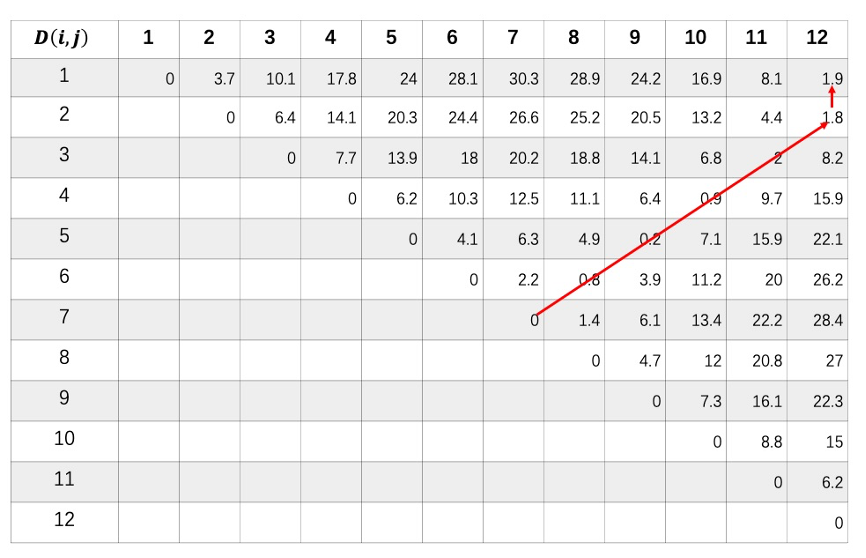
\includegraphics[width=0.86\linewidth]{symmetric_matrix.png}
  \caption{相似度矩阵最优匹配路径示意图}
  \label{fig:symmetric_matrix}
\end{figure}

然而,从$r_1$到$r_k$的有效路径却是指数级的,采用暴力求解的方法不现实。
图~\ref{fig:symmetric_matrix}展示了一个时间序列子段在对称度矩阵上的最优
匹配路径。观察发现,路径R中的点$r_i$对于子段而言是由内向外匹配的。
如果$r_{k+1}$与$r_k=\left(i,j\right)$属于同一个匹配路径中的相邻点,
则$r_{k+1}$只有$(i-1, j),(i-1, j+1),(i, j+1)$这三种可能,
即$r_{k+1}$所表示的匹配范围正好包含了$r_k$的匹配范围,这种匹配顺序
符合了动态规划推导思想的无后效性。进一步,如果约定$D P(i, j)$
为子段$S=\left(p_{i}, p_{i+1}, \dots, p_{j}\right)$的对称度,
则该状态可以由$\{D P(i+1, j), D P(i, j-1), D P(i+1, j-1)\}$中
最小的一个推导而来,这种小区间和大区间的状态具有严格单调性的模型非常
符合区间动态规划算法思想。因此,为了求解式~\ref{eq:best_route},
根据区间动态规划思想构造一个状态矩阵$DP$, 
其中每个元素通过式~\ref{eq:dp_item}得到:

\begin{equation}
  D P(i, j)=D(i, j)+\min \left\{\begin{array}{c}
    D P(i+1, j) \\
    D P(i, j-1) \\
    D P(i+1, j-1)
  \end{array}\right.
  \label{eq:dp_item}
\end{equation}

其中:$1 \leq i \leq j \leq n, D P(i, i)=0, D P(i, i+1)=D(i, i+1)$。
式~\ref{eq:dp_item}表示当前区间的匹配累积距离等于当前点的距离值加上近邻
3个区间匹配累积距离的最小值,$D P(1, n)$便是时间序列子段X的最小匹配累积
代价,即对称度。得到对称度后,为了得到最优匹配路径,
再反向以$r_k$为起点寻找匹配路径。直到$i=j$或者$i=j-1$时,
寻找过程结束,最终得到完整的匹配路径。通过累积计算匹配路径中每对匹配点之间的距离,
可以得到匹配点的距离之和,最终计算得到的$DP(1,n)$即可视为时间序列子段$X$的对称度。

\renewcommand{\algorithmicrequire}{\textbf{输入:}\unskip}
\renewcommand{\algorithmicensure}{\textbf{输出:}\unskip}

\begin{algorithm}
  \caption{单一对称性度量算法$calculate\_single\_symmetry$}
  \label{alg:single_symmetry}
  \small
  \begin{algorithmic}
    \REQUIRE 时间序列子段$X=\left(p_{1}, p_{2}, \dots, p_{n}\right)$
    \ENSURE 对称度$y$

    \STATE $n \leftarrow \left|X\right|$
    \STATE $i \leftarrow 1$
    \WHILE{$i \leq n$}
    \STATE $dp_{i,i} \leftarrow inf$
    \ENDWHILE

    \STATE $i \leftarrow 1$
    \WHILE{$i < n$}
    \STATE $dp_{i,i+1} \leftarrow D\left(p_{i}, p_{i+1}\right)$
    \ENDWHILE

    \STATE $len \leftarrow 3$
    \WHILE{$len \leq n$}
    \STATE $i \leftarrow len$
    \WHILE{$i \leq n-len+1$}
    \STATE $dp_{i,i+len-1} = D\left(p_{i}, p_{i+1}\right)+\min \left(dp_{i,i+len-2},dp_{i+1,i+len-1},dp_{i+1,i+len-2}\right)$
    \ENDWHILE
    \ENDWHILE
    \RETURN $dp_{1,n}$
  \end{algorithmic}
\end{algorithm}

算法~\ref{alg:single_symmetry}给出了
单一对称性度量算法的计算流程。
第1-9行初始化计算长度为1和2的子段对称度,
第10-17行根据式~\ref{eq:dp_item}所示的区间动态规划算法
度量得到给定时间序列子段的对称度。

总结来说,本方法利用区间动态规划的算法思想,
提出了一种兼顾距离相近和形状相似的时间序列子段对称性
度量方法,既避免了对称中心不固定带来的匹配问题,也通过异步匹配
提高了度量的准确性和健壮性,同时,因减少了重复匹配,
也提高了本算法的时间效率。尽管其渐进时间复杂度仍然为
$O\left(w^{2}\right)$,但相比于基于原始和反转时间序列的
DTW距离的相似度度量算法,减少了$50 \%$的重复匹配,
提升了时间序列子段对称度的计算效率。

\section{单一对称度阈值确定算法}

3.1节讲述了单一对称性度量算法,在得到给定时间序列子段的
对称度之后,还需要确定单一对称度阈值,才能判断子段是否具有对称性。
单一对称度阈值用于对单条子段进行分类,
对称度在阈值范围内的子段划分为对称子段,否则划分为非对称子段。
在真实工业场景的数据挖掘中,经常由专家根据领域知识人为确定
先验阈值。例如,在运输车行驶往返形成的时间序列数据中,
由于车道变换导致的相同位置经度变化不会超过0.0001度,
此经验信息可以用为对称子段匹配过程中的单点匹配误差阈值。
尽管使用经验阈值的方式可以高效地对时间序列对称子段进行分类,
但并不是所有来源的数据集都有明确的经验阈值,或者其阈值
只是一个较为模糊的范围,不具有进行对称子段分类的作用。

为了降低不同来源时间序列子段的数据范围差异给对称度阈值确定带来的难度,
用户可以对时序数据进行标准化处理。
标准化处理要求对时间序列子段
$X=\left(\left(t_{1}, x_{1}\right),\left(t_{2}, x_{2}\right), \ldots,\left(t_{n}, x_{n}\right)\right)$
的每个数据点,首先根据公式~\ref{eq:mu}计算数据点的平均值,
再根据公式~\ref{eq:sigma}计算数据点的标准差,
最后按照公式~\ref{eq:standard}对时间序列子段X中所有的数据点进行标准化。
尽管标准化处理在一定程度上消除了各变量在变异程度上的差异,
但并不能对所有来源的数据集确定统一的对称度阈值。
图~\ref{fig:symmetry_diff}展示了对来自UCR的持枪动作位置和
实验室合成信号时间序列子段进行标准化处理的结果。
尽管两条时间序列子段均具有物理上的对称性,属于对称子段,也都经过
了标准化处理,但通过3.1节对称性度量算法计算,
持枪动作位置时间序列子段的对称度为0.025,
而实验室合成信号时间序列子段的对称度为0.01,两者差距较大。
因此,需要设计一种不依赖于领域知识和预处理操作的单一对称度阈值确定算法。
\begin{equation}
  \mu=\frac{\sum_{i=1}^{i=n} x_{i}}{n}
  \label{eq:mu}
\end{equation}
\begin{equation}
  \sigma=\sqrt[2]{\frac{\sum_{i=1}^{i=n}\left(x_{i}-\mu\right)^{2}}{n}}
  \label{eq:sigma}
\end{equation}
\begin{equation}
  y_{i}=\frac{x_{i}-\mu}{\sigma}
  \label{eq:standard}
\end{equation}

\begin{figure}
  \centering
  \subcaptionbox{标准化持枪手势时间序列子段\label{fig:symmetry_diff_gun}}
  {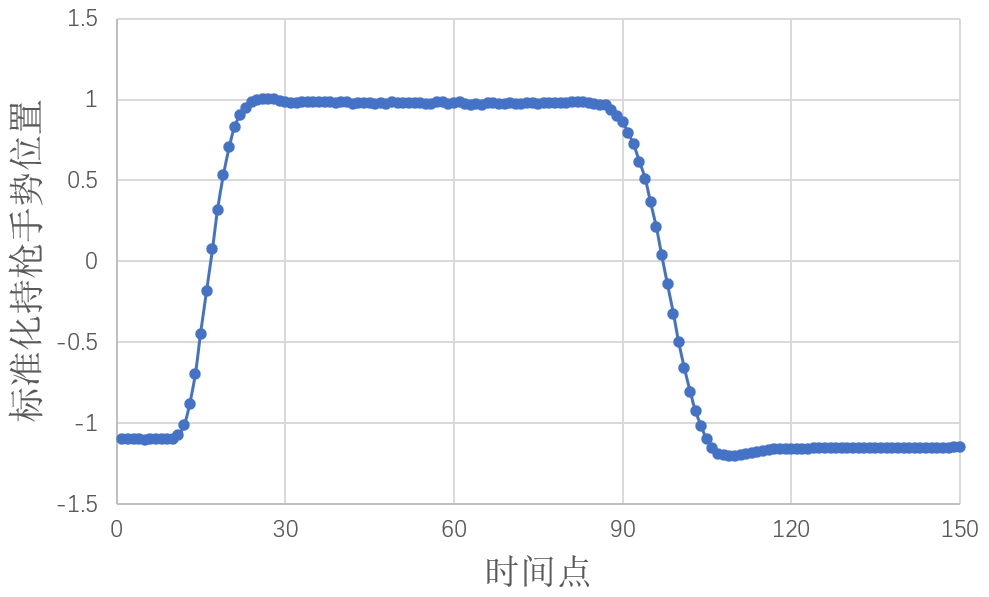
\includegraphics[width=0.43\linewidth]{symmetry_diff_gun.PNG}}
  \subcaptionbox{标准化合成信号时间序列子段\label{fig:symmetry_diff_umd}}
  {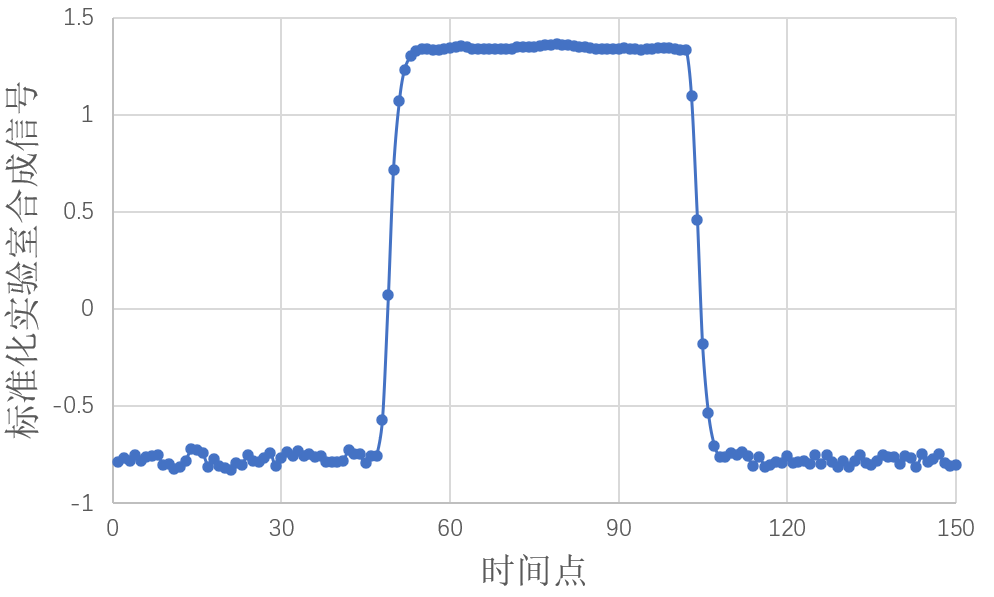
\includegraphics[width=0.43\linewidth]{symmetry_diff_umd.PNG}}
  \caption{不同来源时间序列对称子段对称度差异}
  \label{fig:symmetry_diff}
\end{figure}

考虑到对称度本质上是时间序列子段前后匹配得到的
自相似性结果,因此,对称度阈值必然和子段本身的
差异程度密切相关。如果子段的变化比较平缓,为了
正确判定对称子段,对称度阈值就需要设定的较小。
如果子段变化特别剧烈,相应的在进行对称子段匹配的过程中,
匹配点的差异可能就特别大,因此,对称度阈值也需要
设定的较大。然而,影响对称度阈值高低的关键因素不是标准差
代表的整体子段的差异程度,而是匹配点之间的差异程度。
图~\ref{fig:symmetry_diff}展示的两条时间序列子段
均经过标准化操作,标准差都是1,但两者的对称度却不同。

因此,要根据时间序列子段点匹配的情况确定对称度阈值。然而,
根据子段匹配点之间的距离确定对称阈值具有极大的随机性。
对称度阈值的选取将极大地受对称性度量算法的影响。
因为对称性度量算法将决定子段点的匹配位置。
这样得到的对称度阈值不具有统一性,算法也不具备可迁移性。因此,
对称度阈值的确定还是需要立足子段本身的数据特征。
本文使用在同一个子段中前后相邻点的
差距作为确定对称度阈值的参考。因为对称子段要求前后点相匹配,
符合要求的匹配应该满足匹配点对的距离尽可能小,进而也尽量不要超过匹配点
的近邻点。因此,近邻点距离的统计指标对于对称子段判定
具有很重要的参考意义。
相比中位数,近邻点距离的平均数更能反映时间序列子段的整体变化程度,
也更适用于对单一对称性度量算法计算出来的对称度进行分类。
因为中位数只是考虑了相邻点距离在分布上的中间位置情况,
并未考虑可能存在的距离较大的近邻点。而单一对称性度量
算法是从时间序列子段整体为每个点寻找最佳匹配点,可能包含部分匹配
偏差较大的点,其最终得到的单点对称度从数学意义上来说也是
子段所有匹配点距离的平均数。因此,可以使用式~\ref{eq:threshold1}
所表示的子段近邻点距离的平均值,作为对称子段判定
算法的对称度阈值。为与第4章提出的分段对称度阈值进行区分,
本节提出的单一对称度阈值用$\theta_1$来表示。
对称度阈值需要统一量纲,由于不同来源时间序列对称子段的长度不一致,
因而经对称性度量算法计算出来的对称度
也要求其与子段长度的比值。
\begin{equation}
  \theta_{1}=\frac{\sum_{i=2}^{n}\left|x_{i}-x_{i-1}\right|}{n-1}
  \label{eq:threshold1}
\end{equation}

\section{判定对称子段}
通过单一对称性度量算法计算得到子段对称度之后,就可以
使用领域知识或自定义算法确定的单一对称度阈值对子段进行分类。
在未指定先验阈值的情况下,如果根据公式~\ref{eq:threshold1}
计算得到的单一对称度阈值为$\theta_1$,那么,本文所要判定的
对称子段即是满足公式~\ref{eq:single_symmetry}的时间序列子段。
\begin{equation}
  M = \{X|D(X)\leq\theta_1\}
  \label{eq:single_symmetry}
\end{equation}

综上所述,对称子段判定算法的计算步骤如算法~\ref{alg:single_symmetric}
所示。首先使用单一对称性度量算法计算时间序列子段的
对称度,之后由公式~\ref{eq:threshold1}
计算时间序列子段数据特征相关的单一对称度阈值,
最后通过比较子段对称度是否在阈值范围内
确定其是否属于对称子段。

\renewcommand{\algorithmicrequire}{\textbf{输入:}\unskip}
\renewcommand{\algorithmicensure}{\textbf{输出:}\unskip}
\begin{algorithm}
  \caption{对称子段判定算法$symmtric\_subsegment\_judgment$}
  \label{alg:single_symmetric}
  \small
  \begin{algorithmic}
    \REQUIRE 时间序列子段$X=\left(p_{1}, p_{2}, \dots, p_{n}\right)$
    \ENSURE 布尔型变量,标志时间序列子段$X=\left(p_{1},p_{2},\dots,p_n \right)$是否为对称子段

    \STATE $d \leftarrow calculate\_single\_symmetry(X) $
    \STATE $i \leftarrow 1$
    \WHILE{$i < \left|X\right|$}
    \STATE minus $\leftarrow$ minus $+D\left(p_{i}, p_{i+1}\right)$
    \STATE $i \leftarrow i+1$
    \ENDWHILE
    \STATE $\theta_1 \leftarrow \frac{minus}{n-1}$
    \IF{$d \leq \theta_1 $}
      \RETURN true
    \ELSE
      \RETURN false
    \ENDIF
  \end{algorithmic}
\end{algorithm}


\section{对称子段流式判定算法}
在实际场景中,经常有在对称子段发生时即时报警的应用\cite{2022968}。
金融市场和股票分析是一个对数据的实时性要求很高的场景,
如果在股票指数或价格时间序列出现符合某类子段特征时能及时预报,
将具有极大的应用价值\cite{DBLP:journals/jucs/BeheraDRMD20}。
图~\ref{fig:shanghai_point}展示了
上证指数在2005年至2015年的变化时间序列,
红框所示曲线符合对称子段特征。股票市场中的对称理论是一个
比较小众但成熟的理论,总结为三大对称定律:
其一为价格对称,即股票上涨的价格和下跌的价格相同;
其二为时间对称,股票上涨持续的时间与下跌持续的时间一致;
其三为高低对称,即股票上涨到一半时,后段的走势与前段的走势呈对称状。
这些定律非常符合本文提出的时间序列对称子段特征。
金融时间序列中的对称子段意味着当前经济周期的结束,
如果能成功识别对称子段,在某种意义上则可以成功预测股票的走势,
在经济周期中获得经济效益。然而,金融时间序列往往都有很强的实时性,
数据是实时更新的,不具备第3.1节中已知时间序列子段所有点的情况。
并且,金融时间序列变化快速且剧烈,因此要求算法能快速响应。
基于此,本节通过优化子段对称性度量算法的状态推导,
提高了算法的时间效率,将其扩展到了流式应用场景。
\begin{figure}
  \centering
  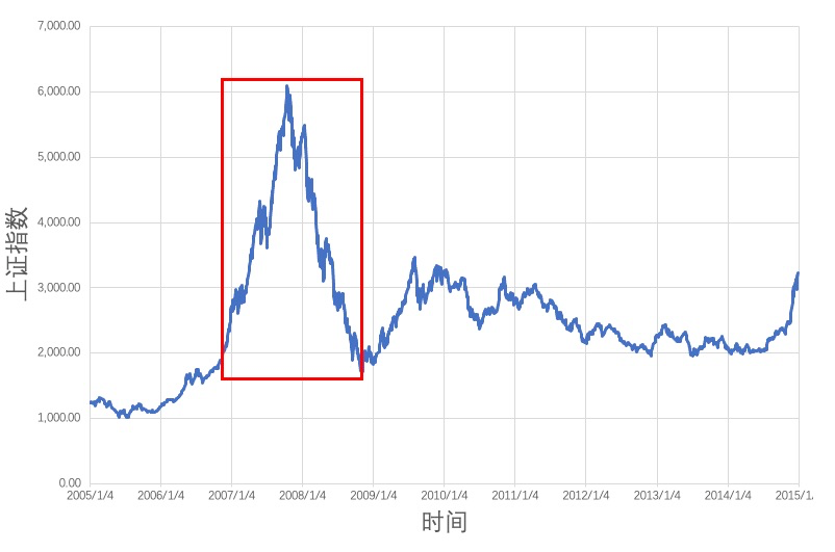
\includegraphics[width=0.76\linewidth]{shanghai_point.png}
  \caption{上证指数自2005年至2015年单日变化情况}
  \label{fig:shanghai_point}
\end{figure}

\subsection{单一对称性流式度量算法}
流式时间序列是一组顺序、大量、快速且连续到达的时间序列数据
\cite{DBLP:conf/apweb/KangWWDW18}。
一般情况下,时间序列数据流可被视为一个随时间延续而无限增长的
动态数据集合。如果能够随着数据点的到来,
不断地对流式数据组成的时间序列子段度量对称性,并在
对称度超过阈值时及时报警,则算法在实时计算领域具有重要的应用价值。
检测流式时间序列子段的对称性需要满足实时性和高效性,
即给定一个实时生成的流式子段$X=(p_1,p_2,\dots,p_t)$,
需要在每个数据点$p_t$生成时,以较高的效率
而不是重新计算的方式检测并度量流式子段$X$的对称性。
由3.1节可知,使用$DP\left(1,t-1\right)$表示流式子段
$S=(p_1,p_2,\dots,p_{t-1} )$的对称度。因此,
当新到来一个数据点$p_{t}$时,可以用公式~\ref{eq:stream_dp}
计算$DP\left(1,t\right)$。然而在该公式中,
由于$p_{t}$是新增点,状态$DP\left(2,t\right)$
尚未计算,不可直接使用。若直接用DTW算法计算流式时间序列子段$X$
与其反转序列的DTW距离作为该序列的对称度,不仅使得对称度结果
偏高,且其时间复杂度又退化为$O\left(t^2\right)$。
因此,需要考虑如何利用已计算的状态优化流式算法。
\begin{equation}
  DP(1, t)=D(1, t)+\min \left\{\begin{array}{c}
    D P(2, t) \\
    D P(1, t-1) \\
    D P(2, t-1)
    \end{array}\right.
  \label{eq:stream_dp}
\end{equation}

图~\ref{fig:latitude_stream_matrix}展示了运煤车单次运输过程
中纬度变化时间序列和单点实时新增时对称度状态推导的变化过程,
通过观察动态规划状态的推导过程可知,当新增一个数据点$p_t$时,
子段$S=\left(p_{1},p_{2},\dots,p_{t-1} \right)$
范围之内的对称度状态不须重新推导。因为根据3.1节介绍的时间序列
子段对称性度量算法的数学性质,该算法满足单调性和连续性,子段
$S$从$p_{1}$到$p_{t-1}$之间的对称度状态$DP\left(i,j\right)$
仍然是由$DP\left(i+1,j\right)$,$DP\left(i,j-1\right)$
和$DP\left(i+1,j-1\right)$推导而来。这三个状态在对称度矩阵
中分别位于$DP\left(i,j\right)$的下方、左方和左下方。
而由图~\ref{fig:latitude_stream_matrix}的状态转移矩阵可知,
当新增数据点$p_t$时,对称度状态矩阵窗口
整体向右下方扩张,并未导致$p_{1}$到$p_{t-1}$之间产生
状态失效,这就使得对称度矩阵内的状态推导顺序仍然有效。并且,
对称性度量算法的起始状态是相邻两点间距离,也不会随着新数据点的
到来而发生改变。在推导顺序和起始状态均未改变的前提之下,只需
计算$DP\left(k,t\right),1\leq k \leq t$,
即图~\ref{fig:latitude_stream_matrix}所示状态转移矩阵的
最后一列状态即可。由状态转移矩阵的转移路径可知,
只需在$O\left(t\right)$的时间内便可计算出$DP\left(k,t\right)$,
相比通过计算原始和反转时间序列的相似性度量对称性的算法大大降低了时间复杂度。
\begin{figure}
  \centering
  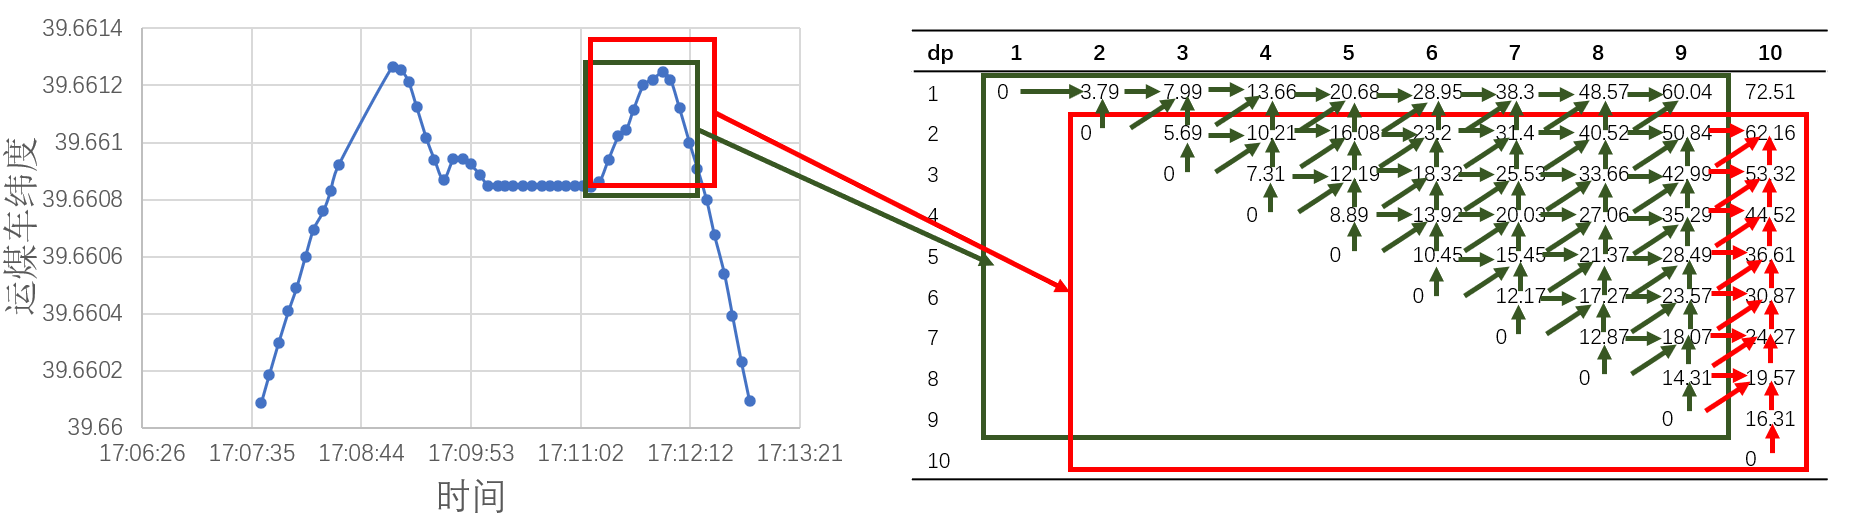
\includegraphics[width=0.92\linewidth]{latitude_stream_matrix.png}
  \caption{运煤车纬度变化与对称度状态转移过程}
  \label{fig:latitude_stream_matrix}
\end{figure}

\subsection{流式判定对称子段}
本节根据子段对称性度量算法在流式数据上的分析和扩展,
提出了相应的流式算法。在流式应用场景中,
触发计算的是新数据点的到达,其他位于窗口内的数据点已经到达
并保存。因此,需要自定义并维护一个队列保存流式时间序列子段$X$,
由历史已经到达的数据点组成,作为流式计算的
状态信息。并且,由图~\ref{fig:latitude_stream_matrix}的
状态转移矩阵可以发现,流式对称子段挖掘算法并不需要利用
完整的对称度矩阵信息,当新增一个数据点$p_t$时,只需要用到
对称度矩阵的最后一列状态来推导和$p_t$相关的状态。
因此,可以使用一维列表$dp$作为保存对称度矩阵的数据结构,
在利用以点$p_{t-1}$为结束点的旧有$dp$计算得到新数据点
$p_t$的相关状态后,用新计算得到的$dp$更新旧有$dp$即可,
进而优化空间复杂度。
此外,由于流式数据是动态、源源不断到来的,子段识别需要实时报警。
因此,可以采用单一对称度阈值确定算法对流式子段进行分类。
总之,对称子段流式挖掘算法只需要
新增数据点$p_t$作为输入,同时保存
流式时间序列子段$X$,流式对称度状态列表$dp$和
流式对称度阈值$\theta_1$作为状态信息。
对于流式时间序列子段$X$,比较其对称度和阈值的数量关系,
输出其是否属于流式对称子段。

\renewcommand{\algorithmicrequire}{\textbf{输入:}\unskip}
\renewcommand{\algorithmicensure}{\textbf{输出:}\unskip}

\begin{algorithm}
  \caption{对称子段流式判定算法$streaming\_symmtric\_subsegment\_judgment$}
  \label{alg:streaming_symmetric_pattern}
  \small
  \begin{algorithmic}
    \REQUIRE 新数据点$p_t$
    \ENSURE 布尔型变量,标志流式时间序列子段$X=\left(p_{1},p_{2},\dots,p_t \right)$是否为流式对称子段

    \IF{$t = 1$}
      \STATE $dp_{1} \leftarrow 0$
    \ELSE
      \STATE $\theta_1 \leftarrow \theta_1+D\left(p_{t}, p_{t-1}\right)$
      \STATE $dp_1^{\prime} \leftarrow 0$
      \STATE $ idx \leftarrow 1$
      \WHILE{$ idx \leq |dp|$}
        \STATE $ idx \leftarrow idx+1$
        \IF{$idx = 2$}
          \STATE $dp_{idx}^{\prime} \leftarrow D\left(p_{t}, p_{t-idx-1}\right)$
        \ELSE
          \STATE $dp_{idx}^{\prime} \leftarrow D\left(p_{t}, p_{t-idx-1}\right)+min(dp_{idx},dp_{idx-1},dp_{idx-1}^{\prime})$
        \ENDIF
      \ENDWHILE
      \STATE $ dp \leftarrow dp^{\prime}$
    \ENDIF
    \STATE 将$p_t$置于流式时间序列子段$X$中
    \IF{$\frac{dp_{t}}{w} > \frac{\theta_1}{w-1}$}
      \RETURN false
    \ELSE
      \RETURN true
    \ENDIF
  \end{algorithmic}
\end{algorithm}

算法~\ref{alg:streaming_symmetric_pattern}
展示了流式时间序列对称子段判定算法
的计算流程,第1-16行在$O(t)$的时间内
流式计算与点$p_t$相关的对称度状态$dp$,
并更新对称度阈值$\theta_1$,
第17行把新数据点放入流式时间序列$X$,
第18-22行
并通过比较流式对称度是否超过对称度阈值,判断是否为对称子段。
分析可知,当每个新数据点到来时,
流式时间序列对称子段判定算法的时间和空间复杂度均为$O(t)$,
远远低于每次都重新计算DTW距离以度量对称性的算法,
具有较高的时间效率和较快的响应速度。
此外,根据第4章的研究,流式判定算法很容易扩展到对称子段挖掘领域,
在结合IoTDB系统实现时具有重要的应用价值。

\section{本章小结}
本章主要介绍了时间序列对称子段判定的整体框架和算法细节。
首先定义了对于单条时间序列子段如何度量对称性,根据最优匹配
和区间动态规划的算法思想设计了单一对称性度量算法。然后,
在先验阈值可能缺省的前提下,3.2节通过分析时间序列子段的
数据特征,根据数据点差分距离的平均值确定了单一子段对称度阈值。
并在3.3节利用阈值过滤得到了对称子段。
最后,本文通过优化对称度计算方式
将对称子段判定算法扩展到了流式数据领域。
根据第5章的实验证明,本节所定义的对称子段判定算法
在不同来源的数据集上具有更高的准确性和鲁棒性。